\documentclass{article}
\usepackage[utf8]{inputenc}
\usepackage{pgfplots}
\usepackage{tikz-3dplot}

\title{Vẽ mặt 3D bằng Tikz}
\author{Your Name}
\date{\today}

\begin{document}

\maketitle

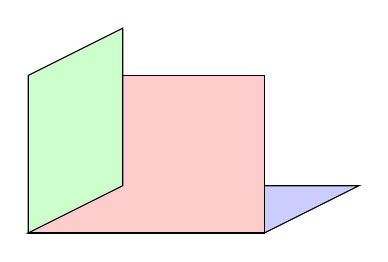
\begin{tikzpicture}[
  x={(1cm,0cm)},
  y={(0.6cm,0.3cm)},
  z={(0cm,1cm)}
]
  % các mặt
  \draw[fill=blue!20] (0,0,0) -- (3,0,0) -- (3,2,0) -- (0,2,0) -- cycle;
  \draw[fill=red!20]  (0,0,0) -- (3,0,0) -- (3,0,2) -- (0,0,2) -- cycle;
  \draw[fill=green!20](0,0,0) -- (0,2,0) -- (0,2,2) -- (0,0,2) -- cycle;
\end{tikzpicture}

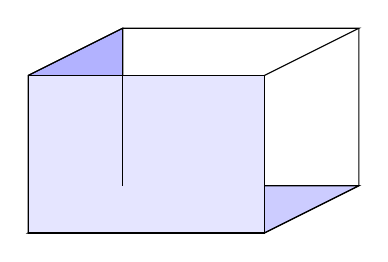
\begin{tikzpicture}[
  x={(1cm,0cm)},
  y={(0.6cm,0.3cm)},
  z={(0cm,1cm)}
]
  \draw[fill=blue!20] (0,0,0) -- (3,0,0) -- (3,2,0) -- (0,2,0) -- cycle;
  \draw[fill=blue!30] (0,0,0) -- (0,2,0) -- (0,2,2) -- (0,0,2) -- cycle;
  \draw[fill=blue!10] (0,0,0) -- (3,0,0) -- (3,0,2) -- (0,0,2) -- cycle;

  % các cạnh nổi
  \draw (3,0,0) -- (3,2,0) -- (3,2,2);
  \draw (0,2,0) -- (0,2,2);
  \draw (3,0,2) -- (3,2,2) -- (0,2,2) -- (0,0,2);
\end{tikzpicture}

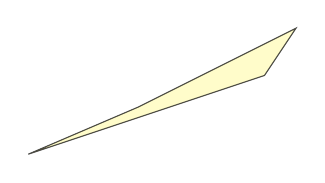
\begin{tikzpicture}[
  x={(1cm,0cm)},
  y={(0.7cm,0.3cm)},
  z={(0cm,1cm)}
]
  \draw[fill=yellow!30, opacity=0.7]
    (0,0,1) -- (3,0,2) -- (2,2,2) -- (0,2,1) -- cycle;
\end{tikzpicture}

\begin{tikzpicture}[scale = 1.2,
  x={(1cm,0cm)},
  y={(0.6cm,0.3cm)},
  z={(0cm,1cm)}
]
  \draw[->] (0,0,0) -- (4,0,0) node[right] {$x$};
  \draw[->] (0,0,0) -- (0,3,0) node[right] {$y$};
  \draw[->] (0,0,0) -- (0,0,3) node[above] {$z$};
\end{tikzpicture}

\tdplotsetmaincoords{80}{120}

\begin{tikzpicture}[tdplot_main_coords]
  \draw[->] (0,0,0) -- (4,0,0);
  \draw[->] (0,0,0) -- (0,3,0);
  \draw[->] (0,0,0) -- (0,0,3);

  \draw[fill=blue!20]
    (0,0,0) -- (2,0,0) -- (2,2,0) -- (0,2,0) -- cycle;
\end{tikzpicture}

\end{document}